\documentclass[conference]{IEEEtran}
\IEEEoverridecommandlockouts
% The preceding line is only needed to identify funding in the first footnote. If that is unneeded, please comment it out.
%\usepackage{cite}
\usepackage{amsmath,amssymb,amsfonts}
%\usepackage{algorithmic}
\usepackage{graphicx}
\usepackage{textcomp}
\usepackage{xcolor}
\usepackage{url}
\usepackage{hyperref}
\usepackage{listings}
\def\BibTeX{{\rm B\kern-.05em{\sc i\kern-.025em b}\kern-.08em
    T\kern-.1667em\lower.7ex\hbox{E}\kern-.125emX}}

\usepackage{acronym}
\newacro{dns}[DNS]{Domain Name System}
\newacro{dot}[DoT]{DNS-over-TLS}
\newacro{doh}[DoH]{DNS-over-HTTPS}
\newacro{doq}[DoQ]{DNS-over-QUIC}
\newacro{odns}[ODNS]{Oblivious DNS}
\newacro{odoh}[ODoH]{Oblivious DoH}
\newacro{dohot}[DoHoT]{DNS-over-HTTPS-over-Tor}
\newacro{dotot}[DoToT]{DNS-over-TLS-over-Tor}
\newacro{dotor}[DoTor]{DNS-over-Tor}
\newacro{sld}[SLD]{Second-Level Domain}
\newacro{tld}[TLD]{Top-Level Domain}
\newacro{rcode}[RCODE]{Return Code}
\newacro{isp}[ISP]{Internet Service Provider}
\newacro{tls}[TLS]{Transport Layer Security}
\newacro{edns}[EDNS]{Extension Mechanisms for DNS}
\newacro{ecs}[ECS]{EDNS Client Subnet}
\newacro{cdn}[CDN]{Content Delivary Network}

\newcommand{\todo}[1]{\textcolor{red}{\texttt{TODO: #1}}}


\begin{document}

\title{
    DoHoT or Not? Tuning Tor Circuits for Anonymous DNS Queries
}

\iffalse
\author{\IEEEauthorblockN{1\textsuperscript{st} Jonathan Magnusson}
\IEEEauthorblockA{\textit{Karlstad University} \\
Karlstad, Sweden \\
jonathan.magnusson@kau.se}
\and
\IEEEauthorblockN{2\textsuperscript{nd} Given Name Surname}
\IEEEauthorblockA{\textit{name of organization (of Aff.)}\\
City, Country \\
email address}
}
\fi
\author{Anonymous Authors}

\maketitle

\begin{abstract}
    Foobookee
\end{abstract}


\begin{IEEEkeywords}
    key, words
\end{IEEEkeywords}

\section{Introduction} \label{sec:intro}

The Domain Name System (\ac{dns}) is a fundamental Internet component that
translates human-readable domain names into IP
addresses~\cite{RFC1034,RFC1035}. Whenever a user attempts to access a website
or online resource, a \ac{dns} query is issued to determine the corresponding
IP address. Despite its essential role, traditional \ac{dns} operates in
plaintext, making it vulnerable to eavesdropping, manipulation, and tracking.

Privacy-preserving protocols such as \ac{doh}~\cite{RFC8484} and
\ac{dot}~\cite{RFC7858} have been developed to address these concerns. These
protocols encrypt \ac{dns} traffic between the client and the resolver,
preventing on-path adversaries from observing or tampering with queries and
responses. While \ac{doh} and \ac{dot} significantly improve confidentiality,
they do not fully address privacy concerns -- especially when the resolver
becomes a point of surveillance or data aggregation.

To further decouple the identity of the client from the \ac{dns} query, more
advanced protocols like \ac{odns}~\cite{ODNS} and \ac{odoh}~\cite{RFC9230} have
been proposed. These protocols introduce cryptographic indirection layers,
ensuring no single server can correlate a query with its origin. However, these
schemes often rely on a limited number of specialized servers and assume that
parties do not collude -- a strong assumption in practice. Moreover, deployment
remains limited, and performance overhead can be substantial.

An alternative approach to achieving strong anonymity and unlinkability is to
route \ac{dns} queries through an anonymity network such as
Tor~\cite{dingledine2004}. Tor is a low-latency, onion-routing network designed
to anonymize Internet traffic by relaying it through multiple volunteer-run
nodes. In particular, Alec Muffett's proposal for \ac{dohot}~\cite{DoHoT}
leverages this infrastructure to anonymize \ac{dns} queries while maintaining
the advantages of encrypted transport.

Despite its privacy benefits, \ac{dohot} and similar approaches have
performance limitations. Tor circuits introduce additional latency due to
multiple hops all over the globe, and variability in relay performance can lead
to inconsistent results. As a result, users must often choose between strong
anonymity and usable performance.

In this study, we aim to explore whether it is possible to configure Tor to
mitigate these performance penalties without sacrificing the security and
privacy guarantees. To do so, we begin by defining the relevant threat models
and outlining the capabilities of potential passive and active adversaries in
the context of encrypted \ac{dns} transport.

Beyond the default Tor configuration, we evaluate the impact of three custom
circuit strategies aimed at improving latency:

\begin{enumerate}
    \item Constraining the EntryNode and/or ExitNode in the \texttt{torrc} file to
        be geographically close to the client.
    \item Using \texttt{carml}~\cite{carml} and \texttt{stem}~\cite{stem} to
        create three-hop and two-hop circuits with randomly selected relays.
    \item Creating three-hop and two-hop circuits with relays that are geographically
        proximate to the client.
\end{enumerate}

To eliminate the effects of caching and to maintain consistency across tests,
we issue queries for uniquely generated \acp{sld} under valid \acp{tld},
expected to return an NXDOMAIN \ac{rcode}. This approach ensures that the
observed latency mainly reflects the path between the client and the resolver
rather than the influence of cache hits or additional authoritative name servers.

Through these measurements, we aim to provide a fair and comprehensive
evaluation of various approaches to anonymizing \ac{dns} queries, with
particular attention to the trade-offs between privacy and performance.
Ultimately, we aim to identify configurations that offer practical improvements
for users who seek strong privacy guarantees without intolerable slowdowns.

\section{Background} \label{sec:background}
Foo

\subsection{DNS}
Queries, Resolvers, Authoritative Name Servers

\subsection{Encrypted DNS Transport}
DNS-over-TLS, DNS-over-HTTP, DNS-over-QUIC, Threat-Model

\subsection{Tor}
Relays, Entry, Middle, Exit, Guards, Onions

\subsection{Anonymous Queries}
Oblivious DNS, Oblivious DoH, DoHoT, Threat-Model



\section{Method} \label{sec:method} Prior work on anonymous \ac{dns} queries
has primarily focused on query latency when comparing against Tor-based
approaches~\cite{RFC9230,kurihara2023muodns,ODNS,xiao2025}. Such comparisons
typically assume the default Tor client configuration (e.g., in as in
DoHoT~\cite{DoHoT}), where circuits consists of three randomly selected relays
(see Section~\ref{sec:bg:tor}). The geographic placement of these relays can
heavily influence latency results. To provide a more complete picture, our
overarching evaluation considers additional dimensions such as the threat model
and deployability, in addition to exploring how we can reduce latency in
Tor-based solutions.

This study is focusing on two approaches for reducing latency in Tor circuits:
controlling the \emph{number} of relays and the \emph{location} of relays. The
default Tor configuration method (\texttt{torrc}) allows users to constrain the
geographic location of entry and exit relays via country codes, but offers no
control over the middle relay. It also does not support building circuits with
fewer than three relays. To overcome these limitations, the Python libraries
\texttt{carml}~\cite{carml} and \texttt{stem}~\cite{stem} are used, which
expose fine-grained control over circuit construction. With these tools, it is
possible specify country codes for the middle relay or omit it entirely (see
Figure~\ref{fig:carml-tor}), enabling the exploration of circuit configurations
that balance latency and anonymity systematically. 

\begin{figure}[h]
    \centering
    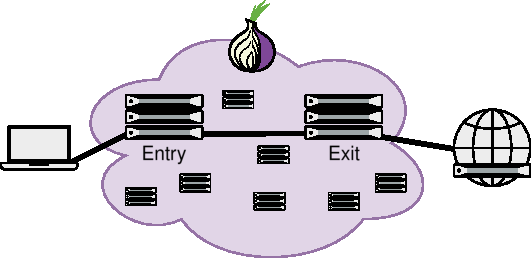
\includegraphics[width=\columnwidth]{img/dns-tor-carml.drawio.pdf}
    \caption{A Tor circuit created with carml and stem, using only an entry
    guard and an exit relay.}
    \label{fig:carml-tor}
\end{figure}

Since the client for the measurements is located in Sweden (country-code:
\texttt{se}), it is estimated that under normal routing conditions the Tor
relays in Sweden places them in close proximity to the client. In
Section~\ref{sec:limit} we address the limitations of Tor relay availability
around the world.

To eliminate the effects of caching and to maintain consistency across tests,
the measurements issue queries for uniquely generated \acp{sld} under a valid
\ac{tld}, which are expected to return an non-existing-domain return code
(NXDOMAIN). The query name consists of
\texttt{prot-method-circuit-i-XXXXXXXX.net}. The first part is the protocol in
use (i.e, dohot, dotor, odoh). The second part is the method for building
circuits (i.e., torrc or carml). The third part represents the built circuit
using the country codes for each relay. A circuit consisting of three
unspecified relays is represented as: \texttt{any2any2any}, while a two relay
circuit contstrained to Sweden is represented as: \texttt{se2se}. In addition
to these parameters an increasing number representing the measurement index
(0-999) as well as a random alphanumeric string are included to ensure that the
query is unique to avoid influence of cache hits. This approach with unique
NXDOMAIN queries ensures that the observed latency mainly reflects the path
between the client and the resolver.

Each configuration is measured 1,000 times with unqiue queries. In each
iteration, we start our measurement container with the specified configuration
and wait until a circuit is established and an arbitrary query receives a
successful response. This prelude ensures that the Tor circuit is fully
established and that we have a functional \ac{dns} resolution over Tor. A query
is then issued for an A record using a unique non-existent domain described
earlier, and the time for the reply to return is measured in milliseconds.
Finally, the container is stopped before the next iteration begins to ensure a
new circuit. The code for the containers and measurement script can be found on
GitHub\footnote{Anonymized for submission}.

For comparison we set up docker containers running \ac{dohot} and
\ac{odoh}. Both of these utilize DNSCrypt-proxy which is a flexible proxy for
\ac{dns} and supports many encryption protocols~\cite{dnscrypt-proxy}.
DNSCrypt-proxy is responsible for listening on a port for client queries and
sending them to the configured anonymization approach. For \ac{odoh} we choose
a proxy in Sweden to mimic the tuned circuit in \ac{dohot}. We decided to pick
a single \ac{doh} provider for our measurements to limit the number of
variables. Our choice of \ac{doh} resolver, Cloudflare's \texttt{1.1.1.1}, is
using anycast which means that the closest from the perspective of our exit or
proxy will be used\footnote{\url{https://developers.cloudflare.com/1.1.1.1/}}.

In addition we also implemented and measured the latency of \ac{dotor}. This is
similar to the Tor-based approach used for comparison with
\ac{odns}~\cite{ODNS} where \ac{doh} is not used. Instead the query is resolved
by the exit relay. Our \ac{dotor} approach relies on directly interfacing with
the Tor client using its extensions to the SOCKS5 protocol, specifically the
RESOLVE command value (0xF0)\cite{tor-socks5}. This allows for sending a domain
to be resolved instead of a destination for the exit relay to connect to. It
should be noted that this approach does not utilize full \ac{dns}-queries at
this level. To interface with the Tor client a python script is instead
utilized to receive and provide dig-compliant DNS queries and their answers.
While negligible in this context, it should be noted that some overhead is
incurred in the process.



\section{Measurement} \label{sec:measurement}
Foo

\section{Discussion} \label{sec:disc}
Our findings demonstrate that \ac{dohot} can achieve significantly improved
\ac{dns} query performance by tuning Tor circuit configurations,
specifically by reducing the number of hops and by geographically localizing
relays. These optimizations suggest practical pathways to making anonymous
\ac{dns} queries more feasible for everyday use, without fundamentally
compromising privacy guarantees.

\subsection{Performance vs. Anonymity Trade-offs}
The results in Section~\ref{sec:measurement} confirm that three-hop Tor
circuits incur higher latency than two-hop configurations. While Tor's design
conventionally mandates three hops to balance trust and anonymity, our threat
model, focused on \ac{dns} query anonymity, shows that omitting the middle
relay (i.e., using two hops) represent a compelling optimization, particularly
in a latency-sensitive context such as \ac{dns}.

Our comparison between \texttt{torrc} and \texttt{carml+stem} configurations
reveals that default Tor path selection tends to outperform manual circuit
configurations due to bandwidth-weighted relay selection. Nonetheless,
\texttt{carml+stem} offers better control over custom circuit construction
where all relays reside within the same geographic region, significantly
reducing inter-relay latency. 

Reducing the number of hops and specifying the geographic location of relays in
\ac{dohot} does not compromise client privacy within the context of our threat
model for anonymous \ac{dns} queries. However, we do not recommend these
configurations for general Tor usage, as they may weaken anonymity guarantees
in broader applications. Additionally, the anonymity of \ac{dns} queries cannot
be assured in the presence of colluding adversaries under a global threat
model.

The \ac{dotor} approach sacrifices control for simplicity and (expected) minor performance gains. 
Allowing the exit-node to perform the DNS-resolution removes all control thereof. 
Anonymity is instead preserved solely by the Tor-circuit. The main drawbacks here are that the 
query itself might still be logged even though it is anonymized. 
Likewise, should an adversary control either node in a circuit consisting only of a guard 
and exit (e.g. se2se) in addition to the network it could theoretically be possible to correlate
the query and the client.

\subsection{DoHoT in Context of Existing DNS Privacy Protocols}
\ac{dohot} offers a compelling alternative to protocols like \ac{odns} and
\ac{odoh}. Unlike these, it does not require new infrastructure or trusted
third parties, leveraging the mature and widely distributed Tor network
instead. Moreover, since \ac{doh} encrypts \ac{dns} queries end-to-end, exit
relays in \ac{dohot} setups are blind to the query contents, mitigating key
privacy concerns noted in prior studies. 

Schmitt~\emph{et al.}~\cite{ODNS} compared traditional \ac{dns} resolution with
DNS resolution over the Tor network using the Alexa top 10,000 domains. Their
results showed a median resolution time of 31.31 ms for traditional \ac{dns},
compared to 276.76 ms over Tor. It is important to note that their evaluation
used standard Tor configurations, where DNS queries are resolved in plaintext
at the exit relay, unlike \ac{dohot}, which encrypts queries end-to-end using
\ac{doh}. In our measurements, the default three-hop \ac{dohot} configuration
yielded a median resolution time of under 200 ms. When using a two-hop circuit
with both relays near the client, the median dropped below 100 ms.

Schmitt~\emph{et al.} briefly discusses the use of \ac{dns} in Tor in contrast
to \ac{odns}, highlighting several limitations. They note that Tor introduces
significant latency, is susceptible to censorship, and that exit relays may be
held accountable for transmitted content. Additionally, exit relay operators
can observe \ac{dns} queries, and \ac{dns} traffic patterns may be
fingerprinted to compromise client anonymity. Since queries in \ac{dohot} are
encrypted, exit relays can only observe a client communicating with a resolver
without visibility into the actual \ac{dns} content. While Tor censorship
remains a persistent challenge, techniques such as bridge relays provide
potential workarounds. 

Singanamalla~\emph{et al.}~\cite{singanamalla2020} evaluated the performance of
\ac{odoh} in a deployment setting, comparing it with several other protocols
including standard \ac{doh}, proxied \ac{doh}, various \ac{odoh}
configurations, DNSCrypt, and \ac{dohot}. They reported an average resolution
time of approximately 300 ms for \ac{odoh}, while \ac{dohot} averaged 696.40
ms. In contrast, our experiments showed a substantially lower average for
\ac{dohot} at 238.11 ms. With a two-hop circuit using relays located in the
same country as the client, the average resolution time was further reduced to
155.54 ms.

\subsection{Limitations}
However, \ac{dohot} still inherits limitations from Tor, including potential
censorship and reliance on public volunteer infrastructure. Compared to
\ac{odns} or \ac{odoh}, which can offer lower latency and are easier to deploy in
centralized environments, \ac{dohot}'s reliance on Tor's ecosystem might hinder
scalability for very high-throughput scenarios.

Our findings indicate that the middle relay in Tor's conventional three-hop
design may not be necessary for anonymous \ac{dns} resolution within the bounds
of a non-colluding adversary model. However, omitting it reduces the diversity
of the path and may weaken anonymity in settings with more powerful or
coordinated adversaries.

Localizing the entry and exit relays to the same geographic region as the
client significantly reduced \ac{dns} query latency. However, narrowing the
relay selection pool may reduce entropy in path selection, potentially
increasing the risk of relay-based correlation attacks. This strategy should be
applied with caution depending on the user's threat model and required
anonymity level.

Our experiments primarily measured \ac{dns} query latency using NXDOMAIN
lookups. This approach removes caching as a variable and does not fully reflect
real-world usage where cache hits are common.


\iffalse
\begin{table}[h!]
    \centering
    \caption{Comparative Evaluation Dimensions}
    \label{tab:comp}
    \begin{tabular}{|c|c|c|c|}
         \hline
         Approach & Latency & Anonymity & Deployability \\\hline
         \hline
         Do\{T,H,Q\} & Low      & None      & High   \\\hline
         ODNS        & Medium   & Medium    & Low    \\\hline
         ODoH        & Low      & Medium    & Medium \\\hline
         DoHoT 1.0   & High     & High      & High   \\\hline
         DoHoT 2.0   & Medium   & High      & High   \\\hline
    \end{tabular}
\end{table}
\fi



\section{Conclusion} \label{sec:conclusion}
We argue that Tor's original threat model for anonymous communication can be
relaxed in the context of anonymous \ac{dns} queries. By reducing circuit length and
constraining relay locations, we achieve substantial latency improvements while
maintaining resistance to collusion attacks. 

Our measurements confirm that these modifications significantly reduce query
latency, demonstrating that two-hop circuits with geographically localized
relays offer a latency-optimized, collusion-resistant alternative for anonymous
DNS resolution.

Finally, we emphasize that evaluating anonymous \ac{dns} schemes requires more
than performance metrics alone. We propose that threat model assumptions and
deployability considerations be treated as equally important dimensions, and
our results illustrate that Tor-based schemes could strike a favorable balance
across all three for the right use case.


\bibliographystyle{plain}
\bibliography{src/ref} % bibtex main to update

\end{document}
